\documentclass{article}
\usepackage{listings}
\usepackage[utf8]{inputenc}
\usepackage{fancyhdr}
\usepackage{xcolor}
\usepackage{caption}
\usepackage{graphicx}
\usepackage{amsmath}
\usepackage{booktabs}
\usepackage{textcomp}
\usepackage{rotating}
\usepackage[english]{babel}

\graphicspath{ {./images/} }

\definecolor{codegreen}{rgb}{0,0.6,0}
\definecolor{codegray}{rgb}{0.5,0.5,0.5}
\definecolor{codepurple}{rgb}{0.58,0,0.82}
\definecolor{backcolour}{rgb}{0.95,0.95,0.92}

\lstdefinestyle{code}{basicstyle=\ttfamily\footnotesize, breakatwhitespace=false, breaklines=true, keywordstyle=\color{magenta},
    commentstyle=\color{codegreen}, keepspaces=true, showspaces=false, showstringspaces=false}

\lstset{style=code}

\pagestyle{fancy}
\fancyhf{}



\rhead{Callum Donovan}
\lhead{Implementing SAT Algorithms in Software}
\rfoot{Page \thepage}
\lfoot{CS-M20 - 1915769}

\title{\bfseries Implementing SAT Algorithms in Software}
\author{Callum Donovan}
\date{September 2020}

\setlength{\parindent}{4em}
\setlength{\parskip}{0.5em}

\begin{document}

\begin{titlepage}
    \begin{center}
        \Large{\bfseries Implementing SAT Algorithms in Software} \\
        \vspace{4cm}
        \begin{center}
            
\includegraphics[scale=0.2]{swan.jpg}
        \end{center}
        \vspace*{\fill}
        \bfseries{\large Callum Donovan \\
            1915769 \\
            September 1, 2020 \\
            Swansea University \\}
    \end{center}
\end{titlepage}

\section{Abstract}
Modern SAT solvers are able to process large SAT data sets quicker than ever before. The research community have been able to assist in the
development of these algorithms since the early 60's, and work is still being done today to improve the performance of these tools. This
paper will be exploring the concepts of a SAT solving algorithm, and how we can translate them into working software tools using modern
programming languages. The selected algorithm is taken from Donald Knuths epic "The Art of Programming", specifically his newest addition "Facsicle 6,
satisfiability". Algorithm D is a simple implementation of a cyclic DPLL SAT solver that utilises specific data structures and backtracking to achieve
modest performance in most use cases. We have implemented this in C++17, and tested it against a small suite of regular SAT problems presented in the DIMACS
format.

\newpage

\thispagestyle{empty}
\tableofcontents

\newpage

\section{Introduction}
In modern computer science, there exist a large set of computational problems that are deemed to be impossible to compute in a reasonable
amount of time. This set of problems, named NP, forms the basis of what a large majority of computer science researchers have attempted to
solve. From the initial scientific labelling of the P and NP set of computational problems in the early 20th century\cite{pvsnp}, there has been
significant time and effort put into discovering the fastest methods in which we can compute these problems. One such instance of these
problems would be the Boolean Satisfiability Problem.

This problem was first proved to be NP-Complete in 1971 by Stephen Cook and Leonid Levin, Cook being the first to publish his paper in
1971\cite{scook}. Levin further improved on Cook's paper by including search problems with the Boolean Satisfiability Problem in his paper published
in the USSR in 1973\cite{levin}. Since those initial findings, the world of NP-Complete problems has expanded significantly and to this day still
proves that there is an ever growing demand for the advantages that improved SAT solving algorithms bring.

Donald Knuth, a well-known computer science researcher from the United States, recently published another volume of his epic work, "The Art
of Computer Programming". In this volume, Knuth described a set of algorithms that can be used to solve SAT formulas. Our goal is to
explore one of Knuth's algorithms and translate it into a simple piece of software using C\texttt{++}. Thus learning more about the ways in which
SAT algorithms can be implemented in software, as well as the methods which can be used to translate it into a program that others can use.

A secondary goal of this project is to explore the concepts that make SAT algorithms efficient when implemented in software. Research that
already focuses on this will be analysed and implemented into the outcome of this project, and further possible improvements will be found
that could be used within the industry.

\newpage
\subsection{Motivation}
The motivation for this project stems from the desire to constantly iterate and improve on existing solutions so that we can do things
faster and more efficiently. The area of SAT solving is extremely important as it provides key solutions to areas of science that rely on
the ability to process data sets quickly. SAT solvers are not only useful in this area of computer science, but are also used across the
field of science in its entirety. SAT solvers can be used to process problems from a multitude of sources, mainly other problems that are
reduced from their respective sets to the CNF SAT formula. Although improvements in this field will do more for NP-Complete problems than
any other sets, they will still provide benefits to problems that are contained in the NP-Hard set. Examples of NP-Hard problems include
protein folding, cryptography, scheduling and many more.

Although there are already existing solutions that are very efficient and more performant than ever before, there is always room for
improvement. This project aims to explore these concepts in which existing solutions can be built upon, and new solutions can be created.
Donald Knuth has proposed a set of algorithms that should be able to efficiently process SAT formulas when implemented in software. We will
be implementing one of these algorithms to study its efficiency when compared to well-known existing solutions. If one of these solutions
proceeds to be substantially efficient in processing the aforementioned SAT formulas, there is a potential for great scientific advancement
in a wide range of fields, as stated previously.

\subsection{Aims}
To reduce the above sections into a more concise format that explains the exact outcomes desired from this project, our aims are as follows:

\begin{itemize}
    \item To research and explore the concepts of SAT solving algorithms, detailing the best possible current methods.
    \item To analyse a SAT solving algorithm as described by Donald Knuth in his book, "The Art of Computer Programming".
    \item To create a C\texttt{++} program that implements the aforementioned algorithm effectively.
    \item To test the C\texttt{++} program to ensure that it can successfully and correctly process CNF SAT formulas.
\end{itemize}

\newpage
\section{Background Research}
In order to fully understand the project that we are undertaking, we must review and analyse existing literature. This literature will form
the basis of the project and will be a guide as to what to expect. There are multiple different components to consider when talking about
both SAT and NP problems, the former of which is contained within the latter. Existing research has already led us to create some of the
best SAT solvers that we could have ever dreamed of, but we cannot settle for what we already have because it may seem good enough. Science
is all about pushing the boundaries of what we already know, and applying the unknown to see what may come of it.

\subsection{Computational Complexity}
To help with understanding the following topics, we will quickly explain the basic concepts of computational complexity. Computational
complexity theory is an area of study that focuses on classifying computational problems according to their difficulty. These classes are
then grouped together by relation to form a scale of computational complexity. Computational problems are problems in which will be solved
by a computer via an algorithm. The most important classes of which are covered in this paper as a foundation for the project that is to be
carried out. A simple representation of the different classes of complexity theory can be shown like in figure 1:

% Don't forget to add a caption and figure / reference!
\begin{figure}[h]
    \caption{Complexity classes visualised \cite{complex}}
    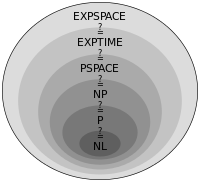
\includegraphics[width=6cm]{complexity.png}
    \centering
\end{figure}

\subsection{P and NP}
Before we can start on the main topic of the project we must first understand the terms that will be used throughout the remainder of this
section. There exists a major unsolved question in computer science, P versus NP. Initially just part of scientific theory within the field
of computational complexity, it became one of the seven Millennium Prize Problems put forward by the Clay Mathematics Institute in 2000.

As we will investigate below, Stephen Cook and Leonid Levin hardened the existence of the P and NP problem independent of each other in the early 1970's. A
simple way to think of the classes P and NP is by their time to find a solution. Problems that reside in the P class can have solutions
found within a reasonable amount of time, or "quickly". Whereas problems that reside in NP cannot have their solutions found within a
reasonable amount of time. But if given the solution to a problem, we can verify the answer quickly. Put simply, P problem solutions are
easy to find, NP problem solutions are easy to check.

\subsection{Cook-Levin Theorem}
To kickstart our development of understanding SAT solvers and their place in the scientific landscape, we must cast our thoughts back to their
initial conception in the early 20th century. Although there had been talk of the concepts of P and NP long before the first concrete
scientific evidence of it, it was not until the publishing of the Cook-Levin theorem in 1971 and 1973 that we would truly expand upon them.
The Cook-Levin theorem is the combination of two papers published at similar times, albeit in separate countries, that described and proved
the same ideas. Stephen Cook published his paper "The Complexity of Theorem Proving Procedures" in the US in 1971\cite{scook}. His paper was the
first to prove that the Boolean Satisfiability Problem was indeed, NP-Complete. Interest in Cook's theory was further increased by Richard
Karp's 1972 paper "Reducibility among Combinatorial Problems"\cite{karp}. Karp expanded upon Cook's initial paper by including a further 20 NP complete
problems, all of which could be reduced to CNF SAT.

Later, in 1975, the scientific interest into P and NP was further increased from the work of Theodore P. Baker, John Gill and Robert
Solovay. Their paper "Relativizations of the P = NP Question" proved that theoretically, solving NP problems in an Oracle machine model
requires exponential time to complete\cite{pnp}. An Oracle machine being an abstract, Turing complete machine that is used to study decision
problems in complexity theory.

A similar result to both Baker, Gill, Solovay and Cook was found in the USSR by Leonid Levin in his 1973 paper "Universal Search
Problems"\cite{levin}. The main difference between the two being the inclusion of search problems by Levin in his paper. Search problems differ from
the problems published by Cook and Karp as they required finding the solution of the problem, as opposed to just confirming it's
existence.

\subsection{CNF SAT}
To further understand the concept of SAT solvers and what they aim to achieve, we must understand both SAT and its most common form, CNF
SAT. The Boolean Satisfiability Problem, often referred to as SAT, is the problem of deciding whether a formula in boolean logic is
satisfiable. A formula can be deemed satisfiable when at least one interpretation of it leads to the entire formula evaluating as true. We
can make this interpretation by assigning true or false values to the logical variables contained within the formula.

When we refer to SAT formulas, we are typically referring to its most common variation CNF-SAT. CNF, or conjunctive normal form, is where
the entire formula is a conjunction of clauses. Where each clause is a disjunction of literals. As stated previously, Stephen Cook's "The
Complexity of Theorem-Proving Procedures" proves that a Boolean Satisfiability Problem formula, expressed in conjunctive normal form, was
indeed the first NP-Complete problem\cite{scook}. An example of a SAT formula in conjunctive normal form is as follows:

\begin{gather*}
    (x\vee y\vee z)\wedge (x\vee y\vee \neg z)\wedge (x\vee \neg y\vee z)\wedge(x\vee \neg y\vee \neg z)\wedge(\neg x\vee y\vee
    z) \\ \wedge(\neg x\vee y\vee \neg z)\wedge(\neg x\vee \neg y\vee z)\wedge(\neg x\vee \neg y\vee \neg z)
\end{gather*}

This particular formula would be called 3-SAT, as each clause contains at most 3 literals. This is one of Karp's 21 NP-Complete problems as
mentioned above and is a good starting point for proving that other problems are NP-Complete via polynomial-time reduction. The main
advantage of using 3-SAT formulas when concerning SAT solvers, is that we want to be able to put our most challenging formulas in their
simplest possible form. Using 3-SAT allows us to analyze and generate better algorithms easier than other formats.

\subsection{How Do SAT Solvers Work?}
Typically the algorithms that existed to solve SAT problems existed mainly to model worst-case scenarios for research. However, since the
turn of the millennium there has been a steady increase in amount of effective and efficient algorithms that can be applied to a large
range of industrial use cases. These algorithms focused on performance and scalability, and their development aided in the research of
many industry centered problems. One such instance of these applications would be their inclusion in the toolbox of electronic design
automation, or EDA.

These SAT solvers are based on developments from well established algorithms and are applied to software libraries ready for production use.
Modern SAT solvers have allowed for dramatic improvements to the speed of EDA, and are able to solve problems containing many thousands of
clauses\cite{sat}.

    \subsubsection{Davis-Putnam-Logemann-Loveland (DPLL)}
    The Davis-Putnam algorithm formed the basis of what modern SAT solvers still use today. In their 1960 paper "A Computing Procedure for
    Quantification Theory"\cite{putnam}, Martin Davis and Hilary Putnam propose an algorithm which includes steps to find the satisfiability of
    propositional ground instances.

    A further refinement using this algorithm was developed in 1962 by Martin Davis, George Logemann and Donald W. Loveland. The
    DPLL algorithm built upon the original by using backtracking for deciding the satisfiability of propositional logic formulae in
    conjunctive normal form\cite{dpll}. As we have established previously, SAT solving has an array of benefits when applied to a multitude of
    different fields. And the DPLL algorithm is still used in modern SAT solvers today, such as Chaff, GRASP and MiniSAT.

    The algorithm works using backtracking. It firsts chooses a literal, assigns a truth value to it, then simplifies the formula. It then
    recursively checks if the simplified formula is satisfiable. If it is, then we deem the formula satisfiable, but if it is not we go back
    and choose the opposite truth literal, simplify then loop recursively through it again until it is satisfiable.

    Modern algorithms are almost always based upon the fundamental operations of this original algorithm. Many of them are purely extensions
    that aim to improve performance in specific scenarios or industrial applications. Even though they may have their own names, they are
    still considered part of the DPLL algorithm group and are deemed as some of the best around.

    \begin{figure}[h]
        \caption{DPLL final implication graph. \cite{dpllgraph}}
        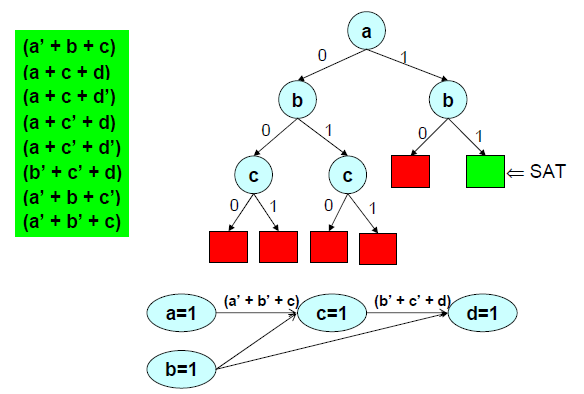
\includegraphics[width=6cm]{Dpll11.png}
        \centering
    \end{figure}

    \subsubsection{Other Algorithms}
    Although most modern SAT solving algorithms are based off of the original DPLL algorithm, there are many who developed their own
    algorithms. These attempt to attack the problem from different angles and employ methods such as local search, or randomization.
    Local search is based on improving the assignment of variables iteratively until the problem is deemed satisfied. However, local search
    is considered an incomplete method, as opposed to DPLL which is considered complete. Incomplete algorithms attempt to find a solution
    the formula, but cannot determine whether the formula is unsatisfiable. An example of a local search based algorithm would be WalkSAT or
    GSAT. Randomized algorithms that use a heuristics based approach include the PPSZ algorithm. These algorithms have been proven to have
    excellent runtime when compared to other algorithms when given a 3-SAT or k-SAT problem\cite{ppsz}.

    \subsubsection{Parallel SAT Solving}
    Since the initial invention of the SAT solving algorithm, there has been leaps and bounds of advancement in computing technology. The
    most important of which being the addition of multiple cores within a single CPU. SAT solvers would typically run on a single physical
    processor, which limited the processing capacity to a single instance of the solver. If the performance of the algorithm is of optimal
    and consistent speed, the time in which a known problem may take to solve will depend on the speed of the single core that is processing
    it. Take for instance the DPLL algorithm, it uses recursion to decide whether a formula is satisfiable or not. The speed at which this
    recursion can run is related to the general performance of the single processor it is on. Before multi-core systems were invented,
    the main goal was to ensure the algorithm could run as fast as possible, using as little resources as possible. CPU's and memory were
    expensive, and thus these algorithms had to make do with what they had. In modern times, we've been able to overcome the majority of the
    cost factor in regards to both memory and processing power. This has led to the creation of SAT solvers that take advantage of
    multi-core systems. These solvers can be grouped into three categories: parallel local search, portfolio and divide-and-conquer. Each
    take advantage of abundant resources in their own ways.

    Portfolio SAT solvers are based on the idea that no SAT solver can be deemed a jack-of-all-trades solution. Each type of SAT solver has
    both strengths and weaknesses that allow it to be good for one type of formula, but bad for another. This has led to an approach where
    the same formula is processed using a collection of different SAT solvers on each processing core, hence the name portfolio. This
    approach can use both different types of SAT solvers, or different configurations of the same SAT solver, to find the best solution in
    the most optimal time. Once one of the SAT solvers reports that they have found the solution and the formula is deemed satisfiable, the
    portfolio halts the process and returns the instance which solved it\cite{parallel}.

    Divide-and-conquer SAT solvers work in the opposite method to Portfolio SAT solvers. Instead of applying multiple different solvers
    against a formula, it is split up and given to each processing core to independently figure out. Although this seems like the most
    logical method of introducing multi-core processing into a problem, it comes with multiple hurdles that have to be offset. The main issue
    being that each search space will vary dramatically in the amount of time it takes to process. This can lead to multiple
    problems and load balancing becomes incredibly complex to achieve\cite{parallel}. A modern approach to combat these problem includes using two types of
    algorithms to deal with the formula in two stages. First the algorithm which is better at small but hard problems will be used to split
    the formula into many small formulas equivalent to the original formula. Each smaller formula will then be given to a CDCL
    algorithm to process independently of the original algorithm. Due to the nature of the smaller formulas still being equivalent to the
    original, if one of the smaller formulas evaluates to TRUE, the original formula is deemed satisfiable\cite{div}.

    Finally, local search algorithms are the hardest to parallelize. One method used includes creating an instance of a local search
    algorithm on one processing core. The initial instance will begin processing the formula, and when it decides to restart its search it
    will produce a configuration that can be passed to a new instance of the algorithm on a new processing core. This configuration will
    build upon the results from the initial instance to increase the chances of finding a solution. This can happen repeatedly over multiple
    processing cores until the algorithm produces a result\cite{local}.

    With the development of even faster processors with more cores becoming accessible to the wider public, we believe that research into
    parallel algorithms would be the best area to focus on. High performance and efficient processors will become even cheaper in the
    following years, and the ability to be able to study the behaviour of these algorithms when applied to many processing cores is becoming
    easier and easier. Even more interestingly, the most recent developments in quantum computing have allowed more research to be put to
    these phenomenal devices. And there is possibility for the technology of quantum computing to become more common in the coming years,
    allowing for them to be used for more trivial operations such as SAT solving.


\subsection{Existing Solutions}
As stated previously, there are multiple SAT solvers publicly available in the form of libraries. They allow anyone to download and use them
for any projects or research they are currently working on. Most of these are well-known in the area of SAT solvers and are already proven
to be of excellent performance when given large formulas. The following are a collection of some of the most renowned libraries used today
in the industry.

Existing libraries typically use the semi standard DIMAC format to ingest formulas. This format consists of three basic rules:

\begin{itemize}
    \item A comment line. Any line beginning with "c" will be seen as a comment line.
    \item A summary line. This line will tell the library about the problem that it is to process. These lines start with a "p", followed by
          the type of problem "cnf", followed by the number of variables and clauses. Depending on the parser used to process these files,
          some may require this line to be first.
    \item A clause line. This line tells the algorithm about each clause contained in the formula. Each clause must be described using
          numbers separated with a single space. The final character denoting the end of the clause is always a 0.
\end{itemize}

This format allows for quick conversion from mathematical format to an ingestible file, and is useful for testing a library with multiple
types of formulas. An example of a clause:

\begin{gather*}
    (x\vee y\vee z)\wedge (x\vee y\vee \neg z)\wedge (x\vee \neg y\vee z)
\end{gather*}

converted into the DIMACS format:

\begin{lstlisting}
    c A formula in DIMACS format
    p cnf 3 3
    1 2 3 0
    1 2 -3 0
    1 -2 3 0
\end{lstlisting}


    \subsubsection{MiniSat}
    The MiniSAT library is a relatively small and fast SAT solver created by Niklas Eén and Niklas Sörensson in 2003. They initially created
    this library as a method to get inexperienced people into the world of SAT solving. Its initial version contained a slim 600 lines of
    code and implemented all of the modern features that were popular at the time. The resulting library was a conflict-driven clause
    learning state of the art SAT solver. The authors further modified the library to compete in more categories in the 2005 SAT
    competition. Even though the extension was considered a "hack" in the eyes of the authors, it proceeded to win silver in a few
    categories and proved to be formidable in categories where it wasn't expected to perform well.

    The final version of MiniSAT is hosted on GitHub for public use, and is freely available for anyone to use and modify to any extent.
    There are modern forks of MiniSAT that are still competing in SAT solver competitions today, thus proving that a well implemented
    library based on a modern extension of the original DPLL algorithm can perform just as well as proprietary industrial solutions.

    MiniSAT includes a simple C\texttt{++} interface, using three vocabulary types:

    \begin{itemize}
        \item \texttt{Minisat::Var} - Used to represent variables
        \item \texttt{Minisat::Solver} - Provides the core functionality of the solver
        \item \texttt{Minisat::Lit} - Used to represent literals in the formula
    \end{itemize}

    These interfaces can be used within a C\texttt{++} program to create a basic implementation that can be passed clauses. In order to pass the
    interface clauses to process, we must include one of MiniSAT's utility types: \texttt{Minisat::vec<T>}. Using these types we can easily
    create a C\texttt{++} script that processes a logical SAT formula:

    \begin{lstlisting}[language=C++]
        #include <iostream>
        #include <minisat/core/Solver.h>

        int main() {
            using Minisat::lbool;
            using Minisat::mkLit;

            // Create solver instance
            Minisat::Solver solver;

            // Create three variables
            auto a = solver.newVar();
            auto b = solver.newVar();
            auto c = solver.newVar();

            // Create three clauses and their included literals
            solver.addClause(mkLit(a), mkLit(b), mkLit(c));
            solver.addClause(mkLit(a), mkLit(b), -mkLit(c));
            solver.addClause(mkLit(a), -mkLit(b), mkLit(c));

            // Begin solving, return the model if satisfiable
            auto sat = solver.solve();
            if (sat) {
                std::clog << "SATISFIABLE\n MODEL FOUND: \n";
                std::clog << "A = " << (solver.modelValue(a) == l_True) << '\n';
                std::clog << "B = " << (solver.modelValue(b) == l_True) << '\n';
                std::clog << "C = " << (solver.modelValue(c) == l_True) << '\n';
            } else {
                std::clog << "UNSATISFIABLE\n";
                return 1;
            }
        }
    \end{lstlisting}

    Further work is required in order to write a script that can solve SAT formulas in CNF, but is still somewhat simple from the use of the
    MiniSAT library and its interface.

\newpage
\section{Project Description}
Expanding further on the aims listed previously, this section will focus on the exact details of the project that we will be undertaking. To
begin, the projects main deliverable will be a working piece of software written in C\texttt{++}. This software should meet the aims of the
project that are listed, and should also coincide with the research undertaken. This project sits between both research and practical, but
the end result should primarily be the software that is to be created. The following will be a guide as to the exact requirements of the
software and what we are expecting to create based on these guidelines. Alongside this, we will list the tools and methods that are to be
used whilst creating this software.

\subsection{Functional Requirements}
The following section describes the expected functional requirements for the project we will be undertaking. There aren't that many
functional requirements that are to be expected when undertaking a project like this, as the resulting software is only going to be a
relatively simple implementation when compared to larger software projects.

    \subsubsection{FREQ1}
    The resulting software should be able to process an input CNF formula in the semi-standard DIMAC format, as described previously.

    \subsubsection{FREQ2}
    The resulting software should be able to evaluate the satisfiability of a simple formula from FREQ1, and return the result
    when found. Simple refers to a formula which most SAT solvers would be able to process in a short amount of time. Result refers to the
    decision returned from the solver that concludes as "SATISFIABLE" or "UNSATISFIABLE".

\subsection{Non-Functional Requirements}
The following section describes the non-functional requirements for the project. These will be auxillary requirements that aren't
necessarily essential for the success of this project. Much like the functional requirements, this project is relatively small compared to
most and doesn't need to have many features or requirements in general.

    \subsubsection{NFREQ1}
    The resulting software should be able to process a complex formula within a reasonable amount of time. Reasonable refers to the length
    of time it takes to return a result when compared to other SAT solvers, i.e. 300 seconds to return "SATISFIABLE".

    \subsubsection{NFREQ1}
    The resulting software should be able to process different forms of SAT formula other than traditional CNF SAT.

\section{Project Plan}
The following section will outline the general plan of the project including methodologies, estimated time plan, tools and risks.
\subsection{Methodology}
There are a large set of software development methodologies available to follow, all of which have their own place in each type of project.
Specifically for this project, it is important to note that the resulting software will not have to adhere to the typical iterative systems
that larger software systems do. This project will be a relatively small, proof of concept that is more focused on the methods in which it
is implemented software-wise. Due to this, we believe that it is not required to use one of the big go-to methodologies that most software
projects will use.

\subsubsection{Chosen Methodology}
The methodology that we have chosen for this project is the Waterfall methodology. Although at first this may seem like a strange choice for
modern software development, we believe that the size and scope of the project does not require the need for a larger, team focused
methodology such as SCRUM. We find that the Waterfall method is a tried and trusted method of developing software based on
concrete requirements with very small teams, or even solo developers.

\subsubsection{Alternative Methodologies}
There are many different types of alternative methodologies that are used widely in todays software landscape. Some of which are
significantly more popular than others due to a number of factors. One example of which would be the Agile software methodology. Within the
Agile methodology, multiple different sub-methodologies have been developed which encompass the basic principles of Agile, whilst adding
their own twists. The basic Agile methodology includes many different techniques to enable a fast, iterative approach to creating software
in a team.

Using one sub-methodology as an example, extreme programming looks more towards solving the issues with changing client requirements along
the development cycle of a software product. In extreme programming, frequent releases over shorter development cycles allow for the
adjustment of requirements to be implemented within the next cycle. This leads to a generally more satisfying outcome for the client, but we
believe that it increases the chance of both feature-creep and incomplete software. We find that this methodology does not suit the very
basic requirements and development plan of the project we are undertaking, and as such was not chosen to be the methodology that we will
follow.

\subsection{Time Plan}
The time plan for this project will span over the next few months. As a simple form of representing the time plant, a Gantt chart has been
created and is displayed on the following page.

\begin{sidewaysfigure}[hbtp]
    \caption{Time plan as formatted as a Gantt chart}
    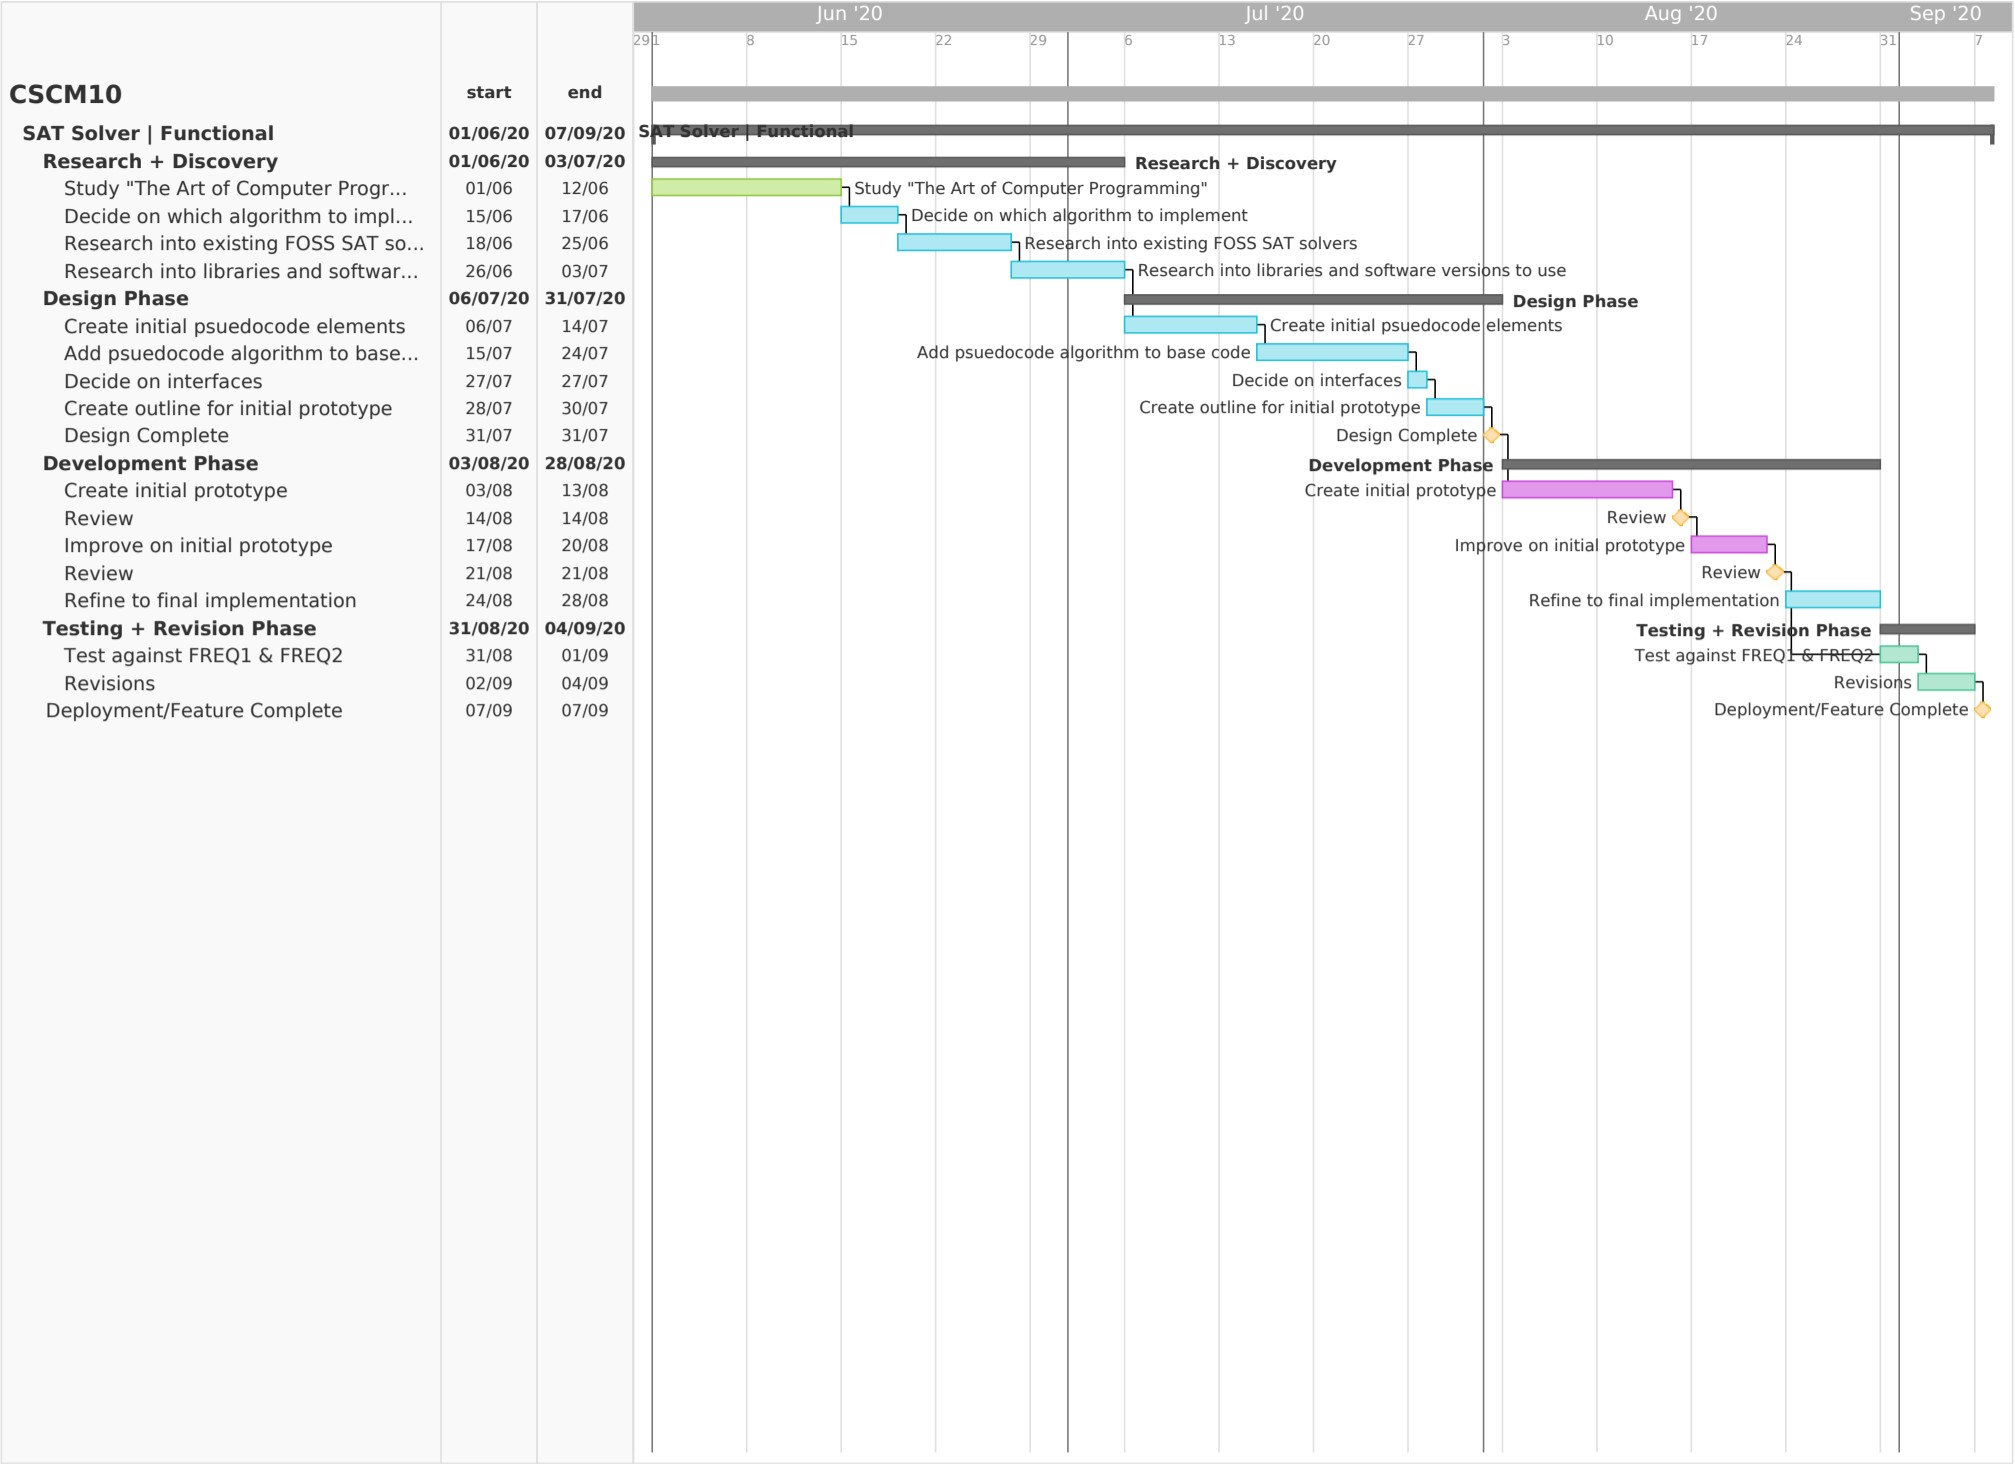
\includegraphics[width=.8\paperwidth]{gantt.jpg}
\end{sidewaysfigure}

\subsubsection{Research + Discovery}
This is the initial development phase of the time plan. It encompasses the
\begin{itemize}
    \item \textbf{Study "The Art of Programming"} - In this task, we will be investigating the Donald Knuth book "The Art of Programming". This will
    be used to form the basis of our understanding of the algorithms that he has created. One of which will be used for this project and
    turned into the C\texttt{++} program.
    \item \textbf{Decide on which algorithm to implement} - Here will will be taking a few days to finalize the algorithm that we want to implement
    the program we are creating for this project.
    \item \textbf{Research into existing FOSS SAT solvers} - At this point we will find and evaluate the existing solutions that are free and open
    source. This is an important step to understand the generic layout of most implementations of SAT solvers in software, and should guide
    us in a general direction that we want to go.
    \item \textbf{Research into existing libraries and software versions to use} - This sounds similar to the previous task, but is instead a further
    research into the potential libraries and software that we will use to build the final program. An example of this would be the
    difference between choosing C\texttt{++} 14 or C\texttt{++} 17.
\end{itemize}

\subsubsection{Design Phase}
In this phase, we will be developing the initial design elements for our program. This will include developing basic psuedocode as a basis
for further development using the programming language of our choice. This phase is important to follow, as it will save lots of time
and effort that otherwise might be wasted in the development phases by dealing with the layout of the code.
\begin{itemize}
    \item \textbf{Create initial psuedocode elements} - Here we will be creating the general structure of the program via the use of
    psuedocode. It will allow the boilerplate code for the final program to be added in quickly without much change.
    \item \textbf{Add psuedocode algorithm to base code} - This will expand on the previous task by adding the algorithm in psuedocode to
    the basic structure we created. This will allow us to fine tune the final overall layout of the program before we being implementing it in
    real code.
    \item \textbf{Decide on interfaces} - This step will decide what interfaces we will be needing to make public for the software to
    function as we intend it to. Much like already existing libraries that include interfaces to interact with when implementing them into a
    program.
    \item \textbf{Create outline for initial prototype} - Finally, we will go into further detail using the initial structure and interface
    decisions to create a final general outline that we will be adhering to when creating the software using the chosen programming
    language.
    \item \textbf{Design complete} - Design work is finalized and collated to be used for initial development phase.
\end{itemize}

\subsubsection{Development Phase}
At this phase we will be starting the initial implementation of the program based on the material and choices we made in the design phase.
This is where the program will begin to get its initial functionality and working prototypes will be made.
\begin{itemize}
    \item \textbf{Create initial prototype} - This is the first step in the development phase and will lay the groundwork for the program
    using the initial designs. Here the boilerplate code and interfaces will be created.
    \item \textbf{Review} - A small review step to ensure that all the design guidelines were followed
    \item \textbf{Improve on initial prototype} - Improvements are made the boilerplate and steps are made towards implementing the initial
    part of the algorithm into actual code. As most of the structure has already been created in the design phase, this should be relatively
    simple.
    \item \textbf{Review} - Another small review to ensure the designs were followed as intended.
    \item \textbf{Refine to final implementation} - Here we will iteratively refine to the final version of the program to ensure it meets
    the initial requirements of the project. This will be the final development step before we move to full testing.
\end{itemize}

\subsubsection{Testing + Revision Phase}
This is the final stage in our development plan and one of the most important. Here we will put the program through its paces to ensure that
it meets the original functional requirements. If time permitted in the development phase, the non-functional requirements will also be
tested.
\begin{itemize}
    \item \textbf{Test against FREQ1 \& FREQ2} - This task will test the program to its full potential against the original criteria as
    described by \textbf{FREQ1} and \textbf{FREQ2}.
    \item \textbf{Revisions} - Any problems or issues found from the full testing will be ironed out and tested again to ensure the program
    is working as intended.
\end{itemize}

At this point, the project should be completed and any relevant material should be collated and added to the submission for review.

\subsection{Tools}
The tool-set that is required for this project is somewhat minimal. Each tool will serve a very particular purpose and no unnecessary tools
will be used for the sake of including more. They are as follows:

    \subsubsection{Code Editor}
    There are a whole plethora of code editors and IDE's that can be used for this project, but in order to keep the project simple and
    portable, we will be using the Visual Studio Code editor. This editor is lightweight and platform agnostic, allowing for it to be
    present on any system that we wish to use. Alongside this, it has a huge extension library that allows for development in almost any
    language a simple task.

    The bare minimum extensions that will be used are as follows:
    \begin{itemize}
        \item C / C\texttt{++}
        \item C\texttt{++} Intellisense
        \item C / C\texttt{++} Compile Run
    \end{itemize}

    These extensions will allow for development on any platform, and the last extension will allow for compilation, running and debug right
    from the editor itself. This will allow for much faster prototyping and debugging when developing.

    \subsubsection{Compiler}
    A compiler is the next important step to consider, especially for this project. Each compiler will vary the types of native libraries
    that are available when developing, and the platform that we are developing on will also guide the choice of compiler. For this project,
    we have chosen to use the MinGW compiler for Windows. It works out of the box without any configuration and allows for development in
    any environment with Windows. It has been proven to be one of the best compilers available and has excellent support and documentation,
    something very valuable when developing prototype software.

\subsection{Risk Analysis}
As this project is quite self-contained and does not require much to get going, the levels of risk are relatively low. We can still find
some risks that may pose a threat to the project progressing if we were to encounter them and how we could mitigate them. These are
displayed in the risk analysis table below.
\begin{itemize}
    \item L \textrightarrow{} Likelyhood
    \item S \textrightarrow{} Severity
    \item D \textrightarrow{} Discoverability
\end{itemize}

% TODO: Figure out why this is being forced on to a new page.
\begin{table}[h]
    \caption{A risk table showing weighting and mitigation.}
    \begin{tabular}{@{}lllllll@{}}
    \toprule
    ID & Title & L & S & D & Total & Mitigation \\ \midrule
    1 &
      \begin{tabular}[c]{@{}l@{}}Bad Time\\ Management\end{tabular} &
      3 &
      8 &
      7 &
      168 &
      \begin{tabular}[c]{@{}l@{}}Follow the provided Gantt chart\\ carefully and ensure tasks are\\  completed to schedule.\end{tabular} \\ \midrule
    2 &
      \begin{tabular}[c]{@{}l@{}}Hardware\\ Failure\end{tabular} &
      3 &
      9 &
      2 &
      54 &
      \begin{tabular}[c]{@{}l@{}}Ensure work is backed up to the\\ cloud and is saved regularly.\end{tabular} \\ \midrule
    3 &
      \begin{tabular}[c]{@{}l@{}}Software\\ Failure\end{tabular} &
      3 &
      10 &
      3 &
      90 &
      \begin{tabular}[c]{@{}l@{}}Ensure libraries and software used\\ is of the most stable version if\\ possible.\end{tabular} \\ \bottomrule
    \end{tabular}
\end{table}
\newpage

% ? We don't necessarily need this section for the final report.
%\section{Conclusion}
%To conclude on this paper, we have discovered and analysed existing literature based on the topic that we are focused on. In this literature
%we have found many different methods in which the problem we are facing has been solved in the past. What we have also found is that there
%exists a plethora of research on ways in which we are able to create fast and efficient SAT solvers, in a surprisingly small amount of code.
%The MiniSAT algorithm continues to be one of the most famous in recent year and still serves as a starting point for beginners in the SAT
%solving arena. Furthermore, we have studied the issues and solutions that plague modern parallel SAT solvers. This gives us a good starting
%point to begin the main part of our project, and solid evidence of methods in which we can ensure our resulting program is fast and
%efficient.

% TODO: Make sure this actually starts on a new page.
\section{Project Overview}
Before we can begin the design and implementation of our project, we must gather a general overview of the work to be done. Following the general timeline
of the Gantt chart we created in the previous sections, our first step is to research into both existing SAT solvers and how they work. Secondly, we must
study the book that we will be taking the algorithm from, Donald Knuths "The Art of Programming", which we will refer to as "TAOP" from now on to simplify
things. In our research phase, we will be able to study how some common SAT solvers are implemented, including data structures that they use, and general
programming constructs that enable the solver to be used effectively and efficiently.

\newpage
\section{Research Phase}
\subsection{TAOP}
\subsection{Algorithms}
\subsection{Existing FOSS Solutions}
\subsection{Libraries and Software}

\newpage
\section{Design Phase}
\subsection{Initial Psuedocode}
\subsection{Implementing Algorithm Psuedocode}
\subsection{Initial Design}
\subsection{Completed Design}

\newpage
\section{Development Phase}
\subsection{Initial Prototype}
\subsection{Review}
\subsection{Further Development}
\subsection{Final Implementation}

\newpage
\section{Testing Phase}
\subsection{Debugging \& Testing}
\subsection{Testing Criteria}
\subsection{Results}

\newpage
\section{Revisions Phase}
% TODO: Include some subheadings for this section?

\newpage
\section{Conclusion}

\newpage
\bibliographystyle{ieeetr}
\bibliography{references}
\end{document}
